\section{Z-position Resolution}
\label{secPositionResolution}

The position resolution of the XENON100 detector is defined by the peak separation efficiency of the S2 peak finder algorithm, and depends on the width of S2 signal, which is energy dependent, and electron drift velocity. In the Monte Carlo simulations with GEANT4, the position resolution is approximated with a step-function, which makes an assumption that events above the assumed value are detected with 100\% efficiency. The energy of individual interactions in each event have been summed up, if they happen within a thin cylinder of liquid xenon in the target volume with the height which equals the assumed position resolution. The 3D vertex of such multiple scattering event has been determined from the positions of all individual scatters weighted by their energies.

The position resolution has been estimated by comparing the energy spectrum and integral rate of single scatter interactions measured in the entire target volume with a $^{137}$Cs calibration source with the expectation from a dedicated Monte Carlo simulation, as shown in Fig.~\ref{figPositionResolution}. The best agreement between the simulation and measurement  is achieved when the position resolution assumed for Monte Carlo is 3~mm. This value has been used for the simulations described in Section~\ref{secCES}, and Chapters~\ref{chERbackground} and \ref{chNRbackground}.

\begin{figure}[!h]
\centering
\subfigure[]{
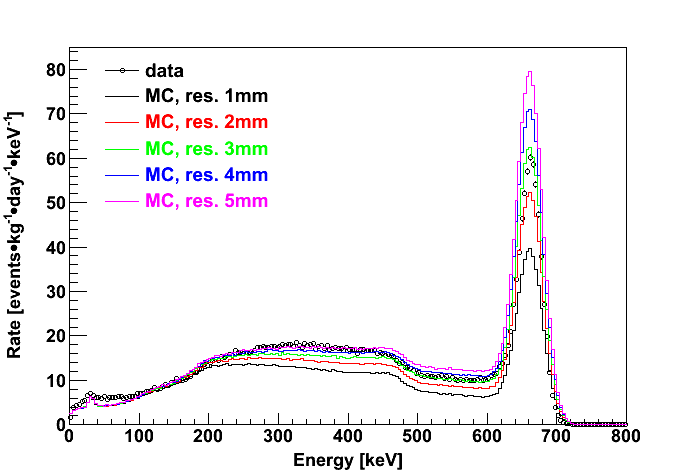
\includegraphics[width=0.475\linewidth]{plots/PositionResolution/CEalex_PassiveVeto_62kg_AllRes.png}
\label{figPositionResolution_1}}
\subfigure[]{
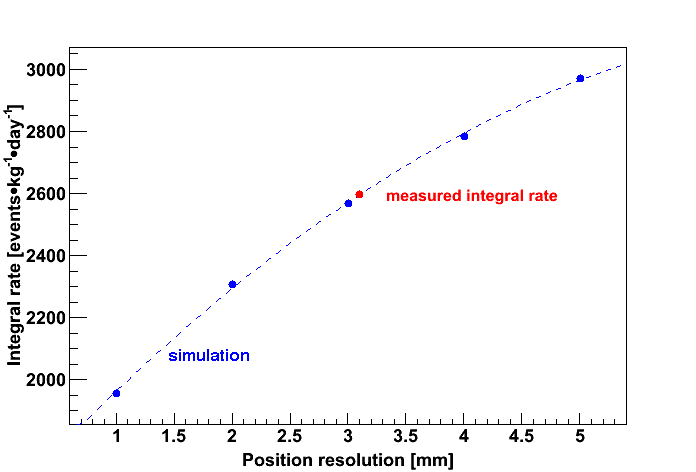
\includegraphics[width=0.475\linewidth]{plots/PositionResolution/RateResolution1.png}
\label{figPositionResolution_2}}
\caption[The $^{137}$Cs spectrum obtained from Monte Carlo data with different position resolutions, and comparison of the integral rate in the simulation and measured data]{The $^{137}$Cs spectrum obtained from Monte Carlo data with different position resolution (a) and comparison of the integral rate of single scatter interactions in the simulation and measured data (b).}
\label{figPositionResolution}
\end{figure}
